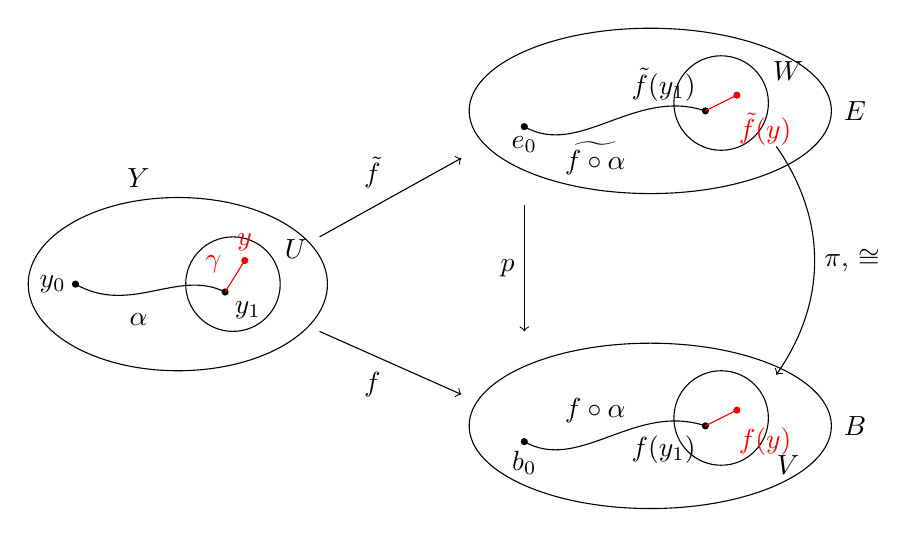
\begin{tikzpicture}
% Y
\draw (0,0) ellipse (1.9 and 1.1);
\node at (-0.5,1.35) {$Y$};
\draw (0.7,0) circle (0.6);
\node at (1.5,0.45) {$U$};
\fill (-1.3,0) circle (1.3pt) node[left] {$y_0$};
\fill (0.6,-0.1) circle (1.3pt) node[below right] {$y_1$};
\draw (-1.3,0) .. controls (-0.6,-0.4) and (0,0.2) .. (0.6,-0.1);
\node at (-0.5,-0.45) {$\alpha$};
\draw[red] (0.6,-0.1) -- (0.85,0.3);
\fill[red] (0.85,0.3) circle (1.3pt) node[above] {$y$};
\node[red] at (0.45,0.25) {$\gamma$};
% E
\draw (6,2.2) ellipse (2.3 and 1.05);
\node at (8.6,2.2) {$E$};
\draw (6.9,2.3) circle (0.6);
\node at (7.75,2.7) {$W$};
\fill (4.4,2.0) circle (1.3pt) node[below] {$e_0$};
\fill (6.7,2.2) circle (1.3pt) node[above left] {$\tilde f(y_1)$};
\draw (4.4,2.0) .. controls (5.1,1.6) and (5.8,2.5) .. (6.7,2.2);
\node at (5.3,1.6) {$\widetilde{f\circ\alpha}$};
\draw[red] (6.7,2.2) -- (7.1,2.4);
\fill[red] (7.1,2.4) circle (1.3pt);
\node[red, below right] at (7.0,2.3) {$\tilde f(y)$};
% B
\draw (6,-1.8) ellipse (2.3 and 1.05);
\node at (8.6,-1.8) {$B$};
\draw (6.9,-1.7) circle (0.6);
\node at (7.75,-2.3) {$V$};
\fill (4.4,-2.0) circle (1.3pt) node[below] {$b_0$};
\fill (6.7,-1.8) circle (1.3pt) node[below left] {$f(y_1)$};
\draw (4.4,-2.0) .. controls (5.1,-2.4) and (5.8,-1.5) .. (6.7,-1.8);
\node at (5.3,-1.6) {$f\circ\alpha$};
\draw[red] (6.7,-1.8) -- (7.1,-1.6);
\fill[red] (7.1,-1.6) circle (1.3pt);
\node[red, below right] at (7.0,-1.7) {$f(y)$};
% maps
\draw[->] (1.8,0.6) -- node[above left] {$\tilde f$} (3.6,1.6);
\draw[->] (1.8,-0.6) -- node[below left] {$f$} (3.6,-1.4);
\draw[->] (4.4,1.0) -- node[left] {$p$} (4.4,-0.6);
\draw[->] (7.6,1.75) to[bend left=35] node[right] {$\pi$, $\cong$} (7.6,-1.15);
\end{tikzpicture}
